\documentclass[runningheads]{llncs}

\usepackage{graphicx}
\usepackage{booktabs}
\usepackage{amsmath}
\usepackage{amssymb}
\usepackage{xcolor}
\usepackage{array}
\usepackage{multirow}
\usepackage{enumitem}
\setlist{itemsep=1pt, topsep=3pt, parsep=0pt, partopsep=0pt}

\begin{document}

\title{PrepAIred: A Specialised Agentic Architecture for Adaptive Multimodal Technical Interview Preparation}
\titlerunning{PrepAIred: A Specialised Agentic Architecture}

\author{Anonymous Author(s)}
\authorrunning{Anonymous et al.}
\institute{Anonymous Institution}

\maketitle

\begin{abstract}
Technical-interview preparation tools typically present fixed-difficulty question pools and coarse, unexplained scoring, with no modular separation between evaluation, adaptation, feedback and execution. We present PrepAIred, a deployed system built as a specialised, orchestrator-coordinated agentic architecture, in which a central orchestrator mediates nine specialised components: a rubric-anchored three-component answer evaluator, a Proximal Policy Optimization (PPO) difficulty controller, a deterministic priority-ordered guardrail layer, a feedback-only large language model, an isolated code-execution sandbox, a speech-analysis pipeline, and supporting state, scoring and timing services. We argue that this decomposition is a research asset, not only an engineering convenience: because difficulty adaptation is split into an independently testable learned component and an independently testable deterministic component, we could design a confirmatory experiment attributing the system's measurable adaptive behaviour to one specific component rather than to the architecture as an undifferentiated whole. We report four such component-attributed findings, each verified directly against the implementation. First, the evaluator correlates with human judgment at Spearman $\rho = 0.3812$ (95\% CI $[0.158, 0.577]$; 3 raters, 64 answers), a moderate, exploratory result. Second, the feedback-only language-model component never computes or adjusts the numeric score, confirmed by direct code-path tracing. Third, a matched multi-seed comparison and a pre-registered confirmatory test attribute the system's measurable difficulty-tracking behaviour to the deterministic guardrail component, not the learned policy, whose marginal contribution is statistically indistinguishable from zero under the same shield -- a finding we trace down to the per-seed and per-turn level. Fourth, boundary testing of the guardrail component found and closed a genuine safety-coverage gap. A formal comparison against a unified single-controller baseline has been designed but, as a disclosed limitation, not yet executed.

\keywords{specialised agentic architecture \and orchestrator-coordinated systems \and adaptive interview preparation \and reinforcement learning \and large language models \and automated answer evaluation \and equivalence testing \and software guardrails}
\end{abstract}

\section{Introduction}

Existing technical-interview preparation tools present a fixed sequence of questions at fixed or self-selected difficulty, score answers through binary or coarse numeric checks where scoring exists at all, and provide no structured explanation of why an answer was scored as it was \cite{key9}. This leaves candidates above the pool's difficulty unchallenged, and others with no scaffolded improvement path. Adaptive testing theory argues that matching item difficulty to an examinee's ability improves measurement efficiency \cite{key9}; the same argument motivates matching interview-practice difficulty to demonstrated skill rather than a static pool. A natural response is to decompose the problem -- evaluation, adaptation, safety, feedback, execution -- into separately testable components under a central controller. This paper asks: where a learned component is paired with a deterministic safety component inside that decomposition, can the architecture's own separability determine \emph{which specific component} is responsible for observed behaviour, rather than this being assumed from the architecture diagram alone?

We present PrepAIred, a deployed adaptive technical-interview system for C-language and data-structures practice, engineered as a specialised, orchestrator-coordinated agentic architecture. A central orchestrator coordinates nine specialised components, each with a distinct responsibility and decision authority: a three-component answer evaluator, a frozen PPO \cite{key6} policy proposing difficulty adjustments, a six-rule deterministic guardrail layer that may override it, a language model used only for narrative feedback, a speech-analysis pipeline, an isolated code-execution sandbox, and candidate-state, scoring and timing services. We report this architecture's full evidence record component by component -- including an unfavourable result for one learned component -- because attributing a finding to one specific component, not the architecture in aggregate, is a direct consequence of a decomposed, orchestrator-coordinated design rather than one fused controller.

A fused implementation that computes a difficulty action in one function cannot, without being rewritten specifically for the purpose, isolate how much of its adaptive behaviour comes from a learned component versus a safety component layered on top of it; the separability built into PrepAIred's components is what later let us design the substitution experiment reported in Sect.~\ref{sec:results}. We treat this as the paper's central methodological point: specialisation's value, in this system, is demonstrated through an attribution result, not assumed from the architecture diagram.

\textbf{Contributions.} (1) A deployed, specialised, orchestrator-coordinated architecture with nine components individually classified by decision authority, not assumed uniformly autonomous. (2) A decomposition-enabled component-level attribution: a matched multi-seed comparison and pre-registered equivalence test isolate the policy's marginal contribution from the guardrail's, finding the former statistically indistinguishable from zero, down to individual seeds and rule activations. (3) An exploratory, disclosed human-correlation validation of the evaluator ($\rho = 0.3812$, 3 raters, 64 answers), with a component ablation and a trivial-baseline comparison. (4) Code-level verification that the feedback-only language model never influences the numeric score, and boundary testing that closed a genuine guardrail safety gap. (5) An explicit, not-yet-executed architectural-comparison design against a unified single-controller baseline.

\textbf{What we do not claim.} Autonomous, peer-to-peer multi-agent collaboration (a dependency audit, Sect.~\ref{sec:architecture}, found none); real-candidate outcome improvement (RL evidence is simulation-based); publication-grade evaluator validation; or that specialisation outperforms a unified controller (designed, Sect.~\ref{sec:future-comparison}, but not run).

The remainder of the paper moves from positioning to evidence: Sect.~2 reviews related work; Sect.~3 describes the architecture; Sect.~4 gives the formulation; Sect.~5 reports results; Sects.~6--7 discuss and conclude.

\section{Related Work and Research Gap}

\textbf{Automated and LLM-assisted scoring.} AutoSCORE \cite{key3} decomposes essay scoring across specialist agents coordinated by a validating agent, outperforming monolithic LLM scoring; independent studies \cite{key1,key2} find LLM-based scoring reliable but prompt- and domain-dependent. PrepAIred's evaluator is structurally similar -- three deterministic, fixed-weight components rather than an LLM judge -- for the same reliability reason: a generative component supplies only feedback text, never the score, verified directly in Sect.~\ref{sec:feedback-verification}.

\textbf{Grounded verification.} Argos \cite{key5} shows that grounding a reward signal in independently checkable evidence, rather than a learned component's own output, reduces hallucination-driven error in agentic RL -- the same principle behind PrepAIred's deterministic scoring path and this paper's component-attribution discipline.

\textbf{Multi-agent coordination evaluation.} MultiAgentBench \cite{key4} establishes milestone-based evaluation of multi-agent coordination quality. We apply its evaluation-methodology principle -- attributing an outcome to a specific internal mechanism, not the system as a whole -- at the orchestrator/policy/guardrail boundary; PrepAIred is orchestrator-coordinated with no verified inter-component arbitration, not a peer-to-peer multi-agent system.

\textbf{Curriculum and difficulty adaptation.} Automated curriculum learning \cite{key12,key13} and intelligent-tutoring knowledge tracing \cite{key10,key11} motivate using a learned policy to sequence difficulty. PrepAIred's RL controller follows this tradition; our contribution is a decomposition-enabled test of whether that component, deployed behind a safety component, performs the identified adaptive work.

\textbf{Multimodal interview analysis.} Prior work analyses interviews from video and multimodal features \cite{key14,key15}. PrepAIred captures audio-derived confidence and hesitation via a dedicated speech component but, by design, no video or facial analysis -- a disclosed scope limitation.

\textbf{Gap addressed.} No prior work reports a specialised, orchestrator-coordinated architecture whose decomposition is used to run a confirmatory test attributing adaptive behaviour to one internal component, paired with an equally disclosed evaluator validation and an explicit, not-yet-executed design for comparing against a unified baseline. This paper reports all three, at a level of granularity -- individual training seeds, individual guardrail rule activations -- that a system-level comparison alone would not expose.

\section{Specialised Agentic Architecture}
\label{sec:architecture}

\subsection{Central Orchestration}

PrepAIred is organised as a hub-and-spoke, orchestrator-coordinated architecture (Fig.~\ref{fig:architecture}).

\begin{figure}[t]
\centering
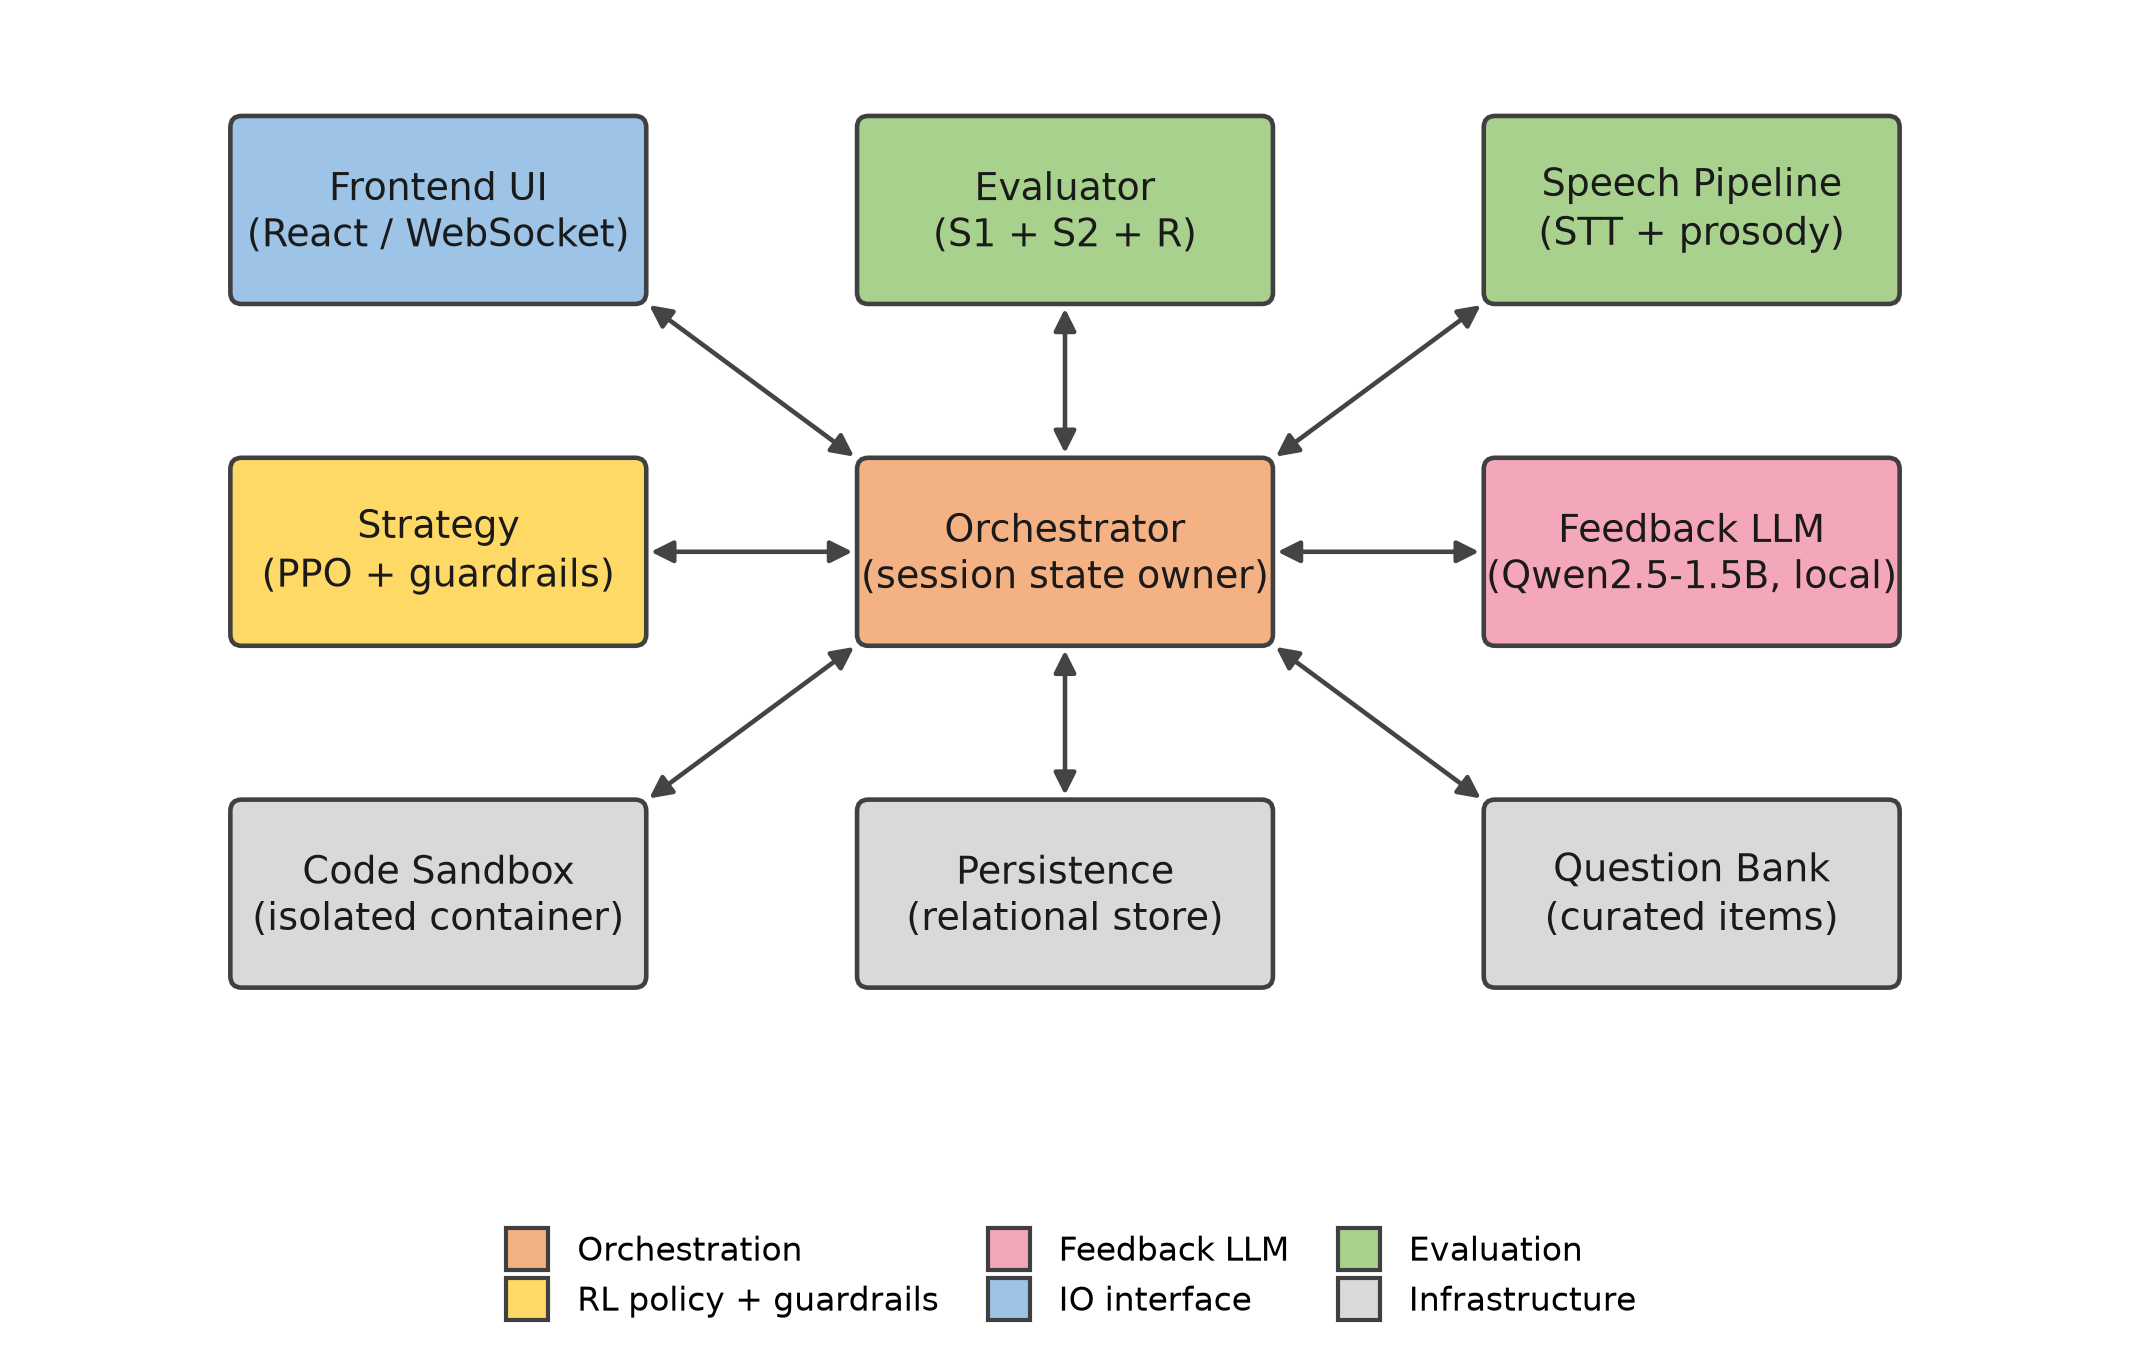
\includegraphics[width=0.66\linewidth]{fig1_architecture.png}
\caption{PrepAIred system architecture. Arrows indicate verified data/control flow between the nine major components; there is no inter-agent arbitration layer.}
\label{fig:architecture}
\end{figure}

A central orchestrator -- one instance per interview session -- owns all session state and mediates every other component: it dispatches each turn event to the relevant component, aggregates outputs into candidate state, and decides the next action. A repository-wide dependency audit, searching every component's source for an import of or call into any sibling component, found zero cross-component edges; the one exception is the feedback component, which issues its own request to the language-model service independently of the orchestrator rather than through it. Coordination here is therefore centralised, not peer-to-peer, and the one exception is explicitly documented rather than smoothed over.

\subsection{Specialised Components and Their Classification}

Table~\ref{tab:classification} classifies each component by decision authority: (A) a genuinely learned or generative decision, (B) specialised logic with bounded, rule-governed authority, (C) a deterministic service with no authority beyond fixed rules, and (D) an ordinary utility with no decision logic at all. No component is classified as a fully autonomous agent negotiating with peers; Category A is reserved for output produced by a trained or generative model, which is the strongest decision-making property this architecture exhibits anywhere.

\begin{table}[t]
\centering
\caption{Component classification by decision authority}
\label{tab:classification}
\small
\begin{tabular}{p{3.1cm}cp{6.3cm}}
\toprule
\textbf{Component} & \textbf{Category} & \textbf{Decision authority} \\
\midrule
Orchestrator & B & Coordinates turns; conditional branching, not learned decisions \\
RL difficulty policy (PPO) & A & Trained forward pass proposes a difficulty action \\
Guardrail layer & C & Six fixed priority-ordered rules may override the proposal \\
Answer evaluator & C & Fixed three-term weighted scoring formula \\
Feedback component (+LLM) & B & Template logic; optional generative narrative text only \\
Code-execution sandbox & C & Fixed compile/execute/compare rules \\
Speech-analysis pipeline & C & Fixed linear signal-processing chain \\
State/scoring/timing services & D & Fixed arithmetic and persistence, no decision logic \\
\bottomrule
\end{tabular}
\end{table}

\subsection{Why Decomposition Matters: Component-Level Attribution}

The architectural choice most load-bearing for this paper is that difficulty adaptation is split into two separately callable components -- the PPO policy (Category A) and the guardrail layer (Category C) -- connected only through the orchestrator, not fused into one function. Because each is callable independently with the same inputs, we could hold the guardrail fixed while substituting the policy with a trivial constant action (Sect.~\ref{sec:results}), isolating which component's output explains the observed behaviour; a fused implementation would not permit this without being rewritten specifically for the experiment. This is the architectural advantage we demonstrate with evidence, not merely assert: not that specialisation improves the outcome, but that it makes the outcome's cause identifiable down to a per-seed, per-turn level of granularity.

The remaining components follow the same rationale: the evaluator, speech pipeline and code sandbox are each independently testable against their own ground truth, which is how the per-component results in Sect.~\ref{sec:results} were obtained, and the feedback component's narrative-only scope is verified by code inspection, never design intent, to never alter the numeric score (Sect.~\ref{sec:feedback-verification}).

\section{Methodology and Formulation}
\label{sec:methodology}

\subsection{Composite Answer Evaluation}

Given a candidate answer split into sentences and a rubric, the evaluator computes three scores. The semantic score $S_1$ averages, over each rubric target $c$, the best cosine similarity between a Sentence-BERT \cite{key7} embedding of $c$ and any candidate sentence:
\begin{equation}
S_1 = \frac{1}{|C|}\sum_{c \in C} \max_{s \in \text{sentences}} \mathrm{cossim}(\mathrm{emb}(c), \mathrm{emb}(s)).
\end{equation}
The concept-coverage score $S_2$ is the fraction of concepts whose best-matching similarity exceeds a threshold $\theta = 0.30$, retrieved via a FAISS index \cite{key8}. The reasoning score $R$ is a fine-tuned cross-encoder's rescaled relevance judgment. $S_2$ is dampened when $R$ is low:
\begin{equation}
S_{2,\mathrm{eff}} = \begin{cases} S_2 & \text{if } R > 0.30 \\ 0.6 \cdot S_2 & \text{otherwise.} \end{cases}
\end{equation}
The final composite score is
\begin{equation}
\mathrm{score} = 0.15 \cdot S_1 + 0.35 \cdot S_{2,\mathrm{eff}} + 0.50 \cdot R
\label{eq:composite}
\end{equation}
(plus a bonus/penalty term), clamped to $[0,1]$ and capped if a mandatory concept is absent. These weights are an engineering default intended to be safety-hardened rather than accuracy-optimal, which directly informs the ablation reported in Sect.~\ref{sec:evaluator-results}; they were not produced by a documented, held-out tuning procedure, and we do not describe them as optimal or learned anywhere in this paper.

\subsection{RL Difficulty Policy and Guardrail Component}

The environment state is $s = [\mathrm{perf}, \mathrm{avg\_perf}, \mathrm{conf}, \mathrm{hes}, \mathrm{progress}, \mathrm{diff}/5] \in [0,1]^6$; the action space is discrete, $a \in \{\text{Easier}, \text{Same}, \text{Harder}\}$. The policy is trained with a hybrid reward
\begin{equation}
r = 0.6 \, r_{\mathrm{decision}} + 0.3 \, r_{\mathrm{outcome}} + 0.1 \, r_{\mathrm{shaping}} + r_{\mathrm{stability}} + r_{\mathrm{critical}},
\end{equation}
where $r_{\mathrm{decision}} = \pm 1$ against a hand-coded rule oracle. The guardrail component, $G(s, a_{\mathrm{proposed}}) \rightarrow a_{\mathrm{final}}$, applies six priority-ordered rules before the action executes, in both training and inference. Because the reward is computed on the \emph{post-guardrail} action, the policy is trained to agree with whichever action the guardrail ultimately selects -- a design detail directly relevant to the attribution result in Sect.~\ref{sec:results}. As a disclosed implementation detail outside this paper's experimental scope, the live orchestrator invokes its own copy of the guardrail rules rather than the canonical training/evaluation module, and the two currently diverge on one rule boundary.

Statistical unit of analysis: five trained policy seeds (42, 123, 456, 789, 999) are each evaluated against five authored personas under five evaluation seeds (1001, 2002, 3003, 4004, 5005); the persona is the primary unit of analysis within each training seed, with the training seed itself a second random factor reported separately rather than pooled. Table~\ref{tab:mae} reports the mean tracking MAE across seeds; Table~\ref{tab:perseed} reports the per-seed breakdown.

\subsection{Feedback Component (Qwen)}
\label{sec:feedback-verification}

A locally hosted Qwen2.5-1.5B-Instruct model (CPU, quantized) generates narrative feedback, hints and follow-up questions, invoked only after the evaluator finalises the score. Every code path that could populate a numeric-score field in its response was traced and found to read that value from the evaluator's own pre-computed result, never to compute it independently; text matching a self-asserted numeric-score pattern is rejected before being shown to the candidate.

\section{Experimental Evaluation and Results}
\label{sec:results}

\subsection{Evaluator Human-Correlation Study}
\label{sec:evaluator-results}

Three raters independently scored 64 constructed candidate answers spanning 8 questions, producing a gold score via mean or adjudicated aggregation. The composite evaluator correlates with the human gold label at $\rho = 0.3812$ (95\% CI $[0.158, 0.577]$; Fig.~\ref{fig:scatter}). Table~\ref{tab:evaluator} reports each component configuration in isolation.

\begin{figure}[t]
\centering
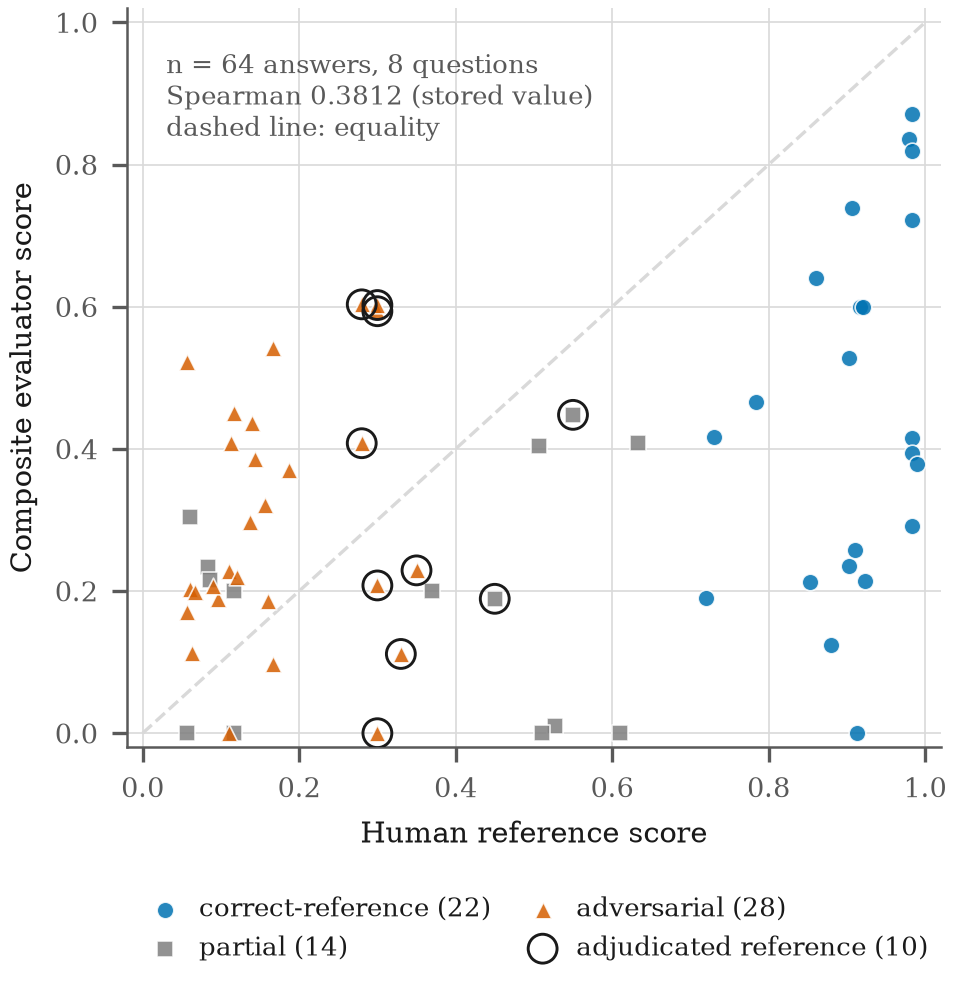
\includegraphics[width=0.5\linewidth]{fig2_evaluator_scatter.png}
\caption{Composite evaluator score vs.\ human reference score, 64 constructed answers. The dashed line marks equality.}
\label{fig:scatter}
\end{figure}

\begin{table}[t]
\centering
\caption{Evaluator correlation with human reference score, by configuration}
\label{tab:evaluator}
\begin{tabular}{lcc}
\toprule
\textbf{Configuration} & \textbf{Spearman $\rho$} & \textbf{95\% CI} \\
\midrule
Full composite & 0.381 & [0.158, 0.577] \\
Cross-encoder $R$ only & 0.483 & [0.246, 0.698] \\
$S_1 + R$ & 0.488 & [0.254, 0.712] \\
$S_1$ (semantic) only & 0.207 & [-0.023, 0.501] \\
Word-count baseline & 0.490 & [0.219, 0.708] \\
\bottomrule
\end{tabular}
\end{table}

The full composite correlates below the cross-encoder alone, consistent with its safety-hardened design discussed in Sect.~\ref{sec:methodology}; a trivial word-count baseline matches the cross-encoder's correlation -- an unflattering result we report rather than omit. We treat this as exploratory evidence for the evaluator component specifically, drawn from a small sample (3 raters, 64 answers across 8 questions), not a validated claim for the architecture as a whole.

\subsection{Feedback-Component Role Verification}

We traced every code path in the feedback component and language-model service that computes or could overwrite the numeric score, confirming neither is ever on that path, and confirmed a run-time guard rejects generated text asserting its own score. This supports Table~\ref{tab:classification}'s classification: the feedback component is Category B (bounded, narrative-only), never Category A for scoring purposes.

\subsection{Component-Attributed Difficulty-Control Comparison}
\label{sec:rl-attribution}

Table~\ref{tab:mae} reports tracking MAE under four conditions, averaged across the five training seeds described in Sect.~\ref{sec:methodology}; lower is better.

\begin{table}[t]
\centering
\caption{Difficulty-tracking error by condition (5 personas $\times$ 5 training seeds $\times$ 5 evaluation seeds)}
\label{tab:mae}
\begin{tabular}{lc}
\toprule
\textbf{Condition} & \textbf{Tracking MAE} \\
\midrule
Fixed difficulty & 1.200 \\
Rule-based heuristic & 0.473 \\
PPO (raw policy) & 0.804 \\
PPO + guardrails & 0.677 \\
\bottomrule
\end{tabular}
\end{table}

The rule-based heuristic outperforms every PPO variant. A pre-registered confirmatory test compared PPO+guardrails against a constant-``Same'' action under the identical guardrail, on a held-out 40-persona grid: the 95\% CI for the difference crosses zero (Fig.~\ref{fig:equivalence}) -- the policy's contribution beyond the guardrail is not statistically distinguishable from zero. Because the two components are independently callable (Sect.~\ref{sec:architecture}), this substitution test required modifying neither component's implementation; we attribute the system's measured adaptive behaviour to the guardrail on this evidence.

\begin{figure}[t]
\centering
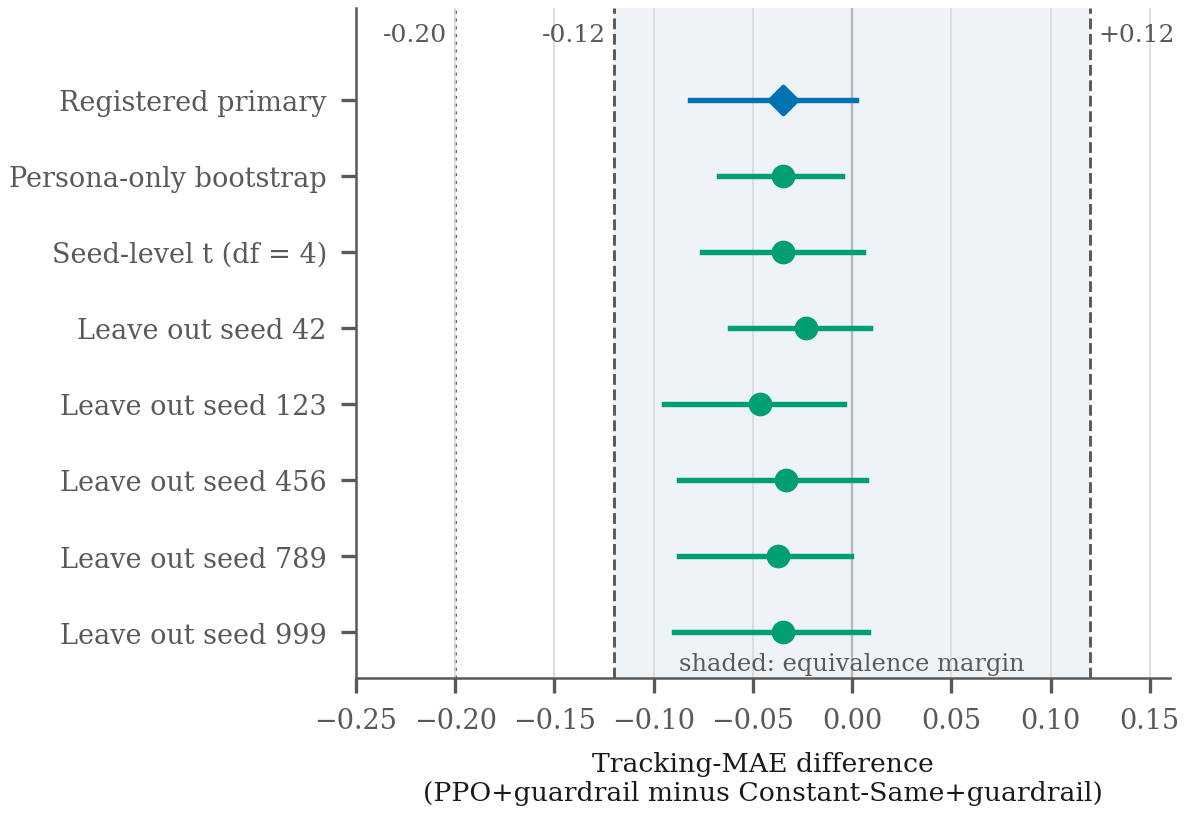
\includegraphics[width=0.5\linewidth]{fig3_equivalence.png}
\caption{Tracking-MAE difference (PPO+guardrails minus constant-action+guardrails) across the primary estimator and six robustness checks. The shaded band is the pre-registered equivalence margin.}
\label{fig:equivalence}
\end{figure}

\textbf{Per-seed breakdown and a disclosed volatility trade-off.} Table~\ref{tab:perseed} reports tracking MAE and session-to-session volatility for each of the five training seeds individually, and compares both against the raw (unguarded) policy and the heuristic baseline. Volatility is the standard deviation of difficulty level across consecutive turns within a session, averaged over sessions. Two findings are visible only at this granularity and would be lost in the pooled mean reported in Table~\ref{tab:mae}: first, every individual training seed's PPO+guardrails MAE (0.673--0.687) clusters tightly around the pooled 0.677, so the pooled result is not an artefact of seed-to-seed cancellation; second, guardrailed PPO is measurably \emph{more} volatile (mean 0.186) than both the raw, unguarded policy (mean 0.078 across the same five seeds) and the heuristic baseline (0.160). The guardrail improves tracking accuracy relative to the raw policy but does so at the cost of more frequent difficulty-level changes session to session -- a trade-off this paper discloses rather than omits, since it qualifies what ``the guardrail accounts for the improvement'' actually means in practice.

\begin{table}[t]
\centering
\caption{Per-training-seed tracking MAE and volatility, PPO+guardrails}
\label{tab:perseed}
\begin{tabular}{lcc}
\toprule
\textbf{Training seed} & \textbf{Tracking MAE} & \textbf{Volatility} \\
\midrule
42 & 0.687 & 0.268 \\
123 & 0.673 & 0.088 \\
456 & 0.676 & 0.208 \\
789 & 0.673 & 0.240 \\
999 & 0.676 & 0.128 \\
\midrule
\textbf{Mean} & \textbf{0.677} & \textbf{0.186} \\
\bottomrule
\end{tabular}

\smallskip
\footnotesize For reference: raw (unguarded) PPO volatility (same 5 seeds) is 0.078; the heuristic baseline's is 0.160.
\end{table}

\textbf{Guardrail intervention accounting.} Because the guardrail is independently callable, we can report how often it actually changes behaviour, not just infer this from the outcome metric. Across the five training seeds (1\,250 turns, 250/seed), a guardrail rule activated on 563 turns (45.0\%; per-seed 122, 101, 115, 120, 105), but 464 of those left the action identical to PPO's own proposal: only 99/1\,250 turns (7.9\%) had a final action differing from PPO's proposal (41/125 sessions had at least one). ``Active on nearly half of all turns'' and ``changes the outcome on one turn in thirteen'' are both true; reporting only the first would overstate the guardrail's footprint relative to what Sect.~\ref{sec:rl-attribution} shows about its necessity.

\subsection{Guardrail Component Boundary Verification}

Boundary testing found performance scores in $[0.30, 0.40)$ unguarded against a policy-proposed escalation; a single-condition threshold widening closed the gap (13/13 boundary cases passing, zero regressions across 283 tests). This defect and fix are specific to the guardrail component in isolation, found by testing its own rule boundaries directly rather than the system end-to-end -- a direct benefit of independent callability.

\subsection{System and Component-Level Testing Summary}

A broader testing programme exercised the orchestrator's dispatch logic, API contract, database integrity, adversarial input handling, and sandbox configuration; 264/283 tests pass (93.3\%), with all 19 remaining failures traced to one unavailable external dependency or one pre-existing, unrelated issue. A later pass re-ran the full suite with zero regressions, confirmed via hash recomputation that the deployed and Sect.~\ref{sec:rl-attribution}-evaluated PPO checkpoints are distinct artefacts, and passed Gymnasium's standard environment check. Table~\ref{tab:testing} summarises this evidence.

\begin{table}[t]
\centering
\caption{System and post-deployment verification evidence, by component}
\label{tab:testing}
\small
\begin{tabular}{p{3.9cm}p{4.3cm}p{3.1cm}}
\toprule
\textbf{Component / check} & \textbf{Method} & \textbf{Result} \\
\midrule
API contract & Direct test-client calls & 7/7 pass \\
Adversarial input (evaluator) & 10 edge-case texts & 10/10, no crash \\
DB integrity (state service) & Live-store inspection & 0/52, 0/26 orphaned \\
Sandbox configuration & Code inspection & All flags present \\
Frontend & Automated UI suite & 28/28 pass \\
Full regression, pre/post-fix & Re-run after 3 fixes & 264/19/15, zero regressions \\
Gymnasium \texttt{check\_env()} & Standard interface check & Passed, no warnings \\
PPO checkpoint identity & Hash recomputation & Deployed/evaluated confirmed distinct \\
\bottomrule
\end{tabular}
\end{table}

\subsection{Architectural Comparison: Status and Design}
\label{sec:future-comparison}

A formal comparison between this architecture and a unified single-controller baseline -- same underlying models and services, coordinated by one controller instead of several specialised classes -- has been fully designed (fairness checklist, 17-category benchmark, primary/secondary metrics, statistical plan) but \textbf{not} executed: no baseline is implemented and no comparative result exists at the time of writing. We report this as a limitation, not as an experimentally shown advantage.

\section{Discussion}
\label{sec:discussion}

The evidence in Sect.~\ref{sec:results} supports three claims. First, decomposing difficulty adaptation into a learned-policy and a deterministic-guardrail component let a pre-registered test identify which one is responsible for the system's adaptive behaviour -- the guardrail, not the policy -- traced down to individual seeds and rule activations, not just a pooled number. This is a benefit of specialisation (attributability), not a claim of superior performance from either mechanism. Second, scoping the language-model component to narrative generation only, and verifying that by code inspection rather than design intent, shows a component's authority can be bounded and checked -- harder in a fused implementation with no seam to inspect. Third, central orchestration integrates these components across turns, modalities and failure conditions, which Sect.~\ref{sec:results}'s testing confirms works at the measured scope. The per-seed volatility finding (Table~\ref{tab:perseed}) qualifies the first claim: the guardrail's accuracy gain over the raw policy is not free -- guardrailed PPO is roughly $2.4\times$ as volatile session to session as the raw policy, and more volatile than the heuristic -- a trade-off a candidate would notice as changing difficulty levels, not only as the aggregate error in Table~\ref{tab:mae}.

This evidence does not support a claim that the architecture outperforms a unified controller end-to-end (Sect.~\ref{sec:future-comparison}, not run), that PrepAIred is a multi-agent system of peers (Sect.~\ref{sec:architecture} found none), or that the evaluator is validated at publication-grade confidence (Sect.~\ref{sec:evaluator-results}'s sample is small and exploratory, and the cross-encoder's fine-tuning provenance is incompletely documented -- an open limitation, not resolved by omission). The multimodal evidence is similarly partial: audio-derived signals only, no video/facial channel as in \cite{key14,key15} -- a scope decision, not an oversight. The defensible contribution is narrower than ``specialisation helps'' but substantive: decomposition under central orchestration made a component-level attribution finding obtainable at all, made a safety-component defect identifiable and fixable in isolation, and exposed a volatility trade-off a system-level metric alone would have hidden.

\section{Conclusion and Future Work}

We presented PrepAIred as a specialised, orchestrator-coordinated agentic architecture and reported its evidence record component by component, with uniform rigour regardless of outcome: an exploratory evaluator correlation; a feedback-only language model verified, not merely claimed; a decomposition-enabled attribution of adaptive behaviour to the deterministic guardrail, down to the per-seed and per-turn level with a disclosed volatility trade-off; and a guardrail boundary fix. Future work: executing the designed single-controller comparison (Sect.~\ref{sec:future-comparison}); a larger evaluator validation study; bounding the cross-encoder's fine-tuning provenance; extending speech analysis toward the video-based signals in \cite{key14,key15}; and a reward trained directly against the tracking metric.

\subsection*{Declaration of AI tool use} Large language model-based tools were used during implementation and manuscript preparation; every quantitative result was independently verified by the authors against stored experimental artefacts before inclusion.

\bibliographystyle{splncs04}
\bibliography{references}

\end{document}
